\documentclass[11pt]{article}

\setlength{\textwidth}{6in}
\setlength{\oddsidemargin}{0.25in}
\setlength{\textheight}{9.0in}
\setlength{\topmargin}{-0.75in}

\input{../common/common-defs}
\usepackage{graphicx}
\usepackage{listings}

\title{VProc protocol}
\author{The Manticore Group}
\date{Draft of \today}

\begin{document}
\maketitle

\section{Overview}
This document describes the protocol for managing vprocs.

\section{Signaling \& sleeping}\label{sec:signaling-and-sleeping}
This section presents two alternative signaling protocols for vprocs.
Both protocols have their advantages, and this section makes an attempt to understand
which is most appropriate for the Manticore implementation.
The rest of this section is structured as follows.
In this secion we outline the interface and semantics of the protocol.
Section \ref{sec:protocol1} describes the first protocol, and section
\ref{sec:protocol2} describes the second protocol.
Then \secref{sec:conclusion} compares the protocols.

\paragraph{Signals}
A signal is a fiber paired with fiber-local storage.
To handle a signal, a vproc initializes the fiber-local storage and runs the fiber to completion.

\paragraph{Landing pad}
The \emph{landing pad} is a lock-free linked list of incoming signals.
Each vproc owns a landing pad, and has access to all the other remote landing pads.
The landing pad supports two operations.
\begin{enumerate}
  \item Push a message on a remote landing pad.
  \item Pop all messages from the local landing pad.
\end{enumerate}

\paragraph{Sleeping}
When there is nothing to do, a vproc enters a temporary sleeping state, which lasts until a
signal arrives on the landing pad or a global garbage collection is initiated by some other
vproc.
We avoid busy waiting by waiting on a condition variable provided by the Pthreads
library.
Unfortunately, the fact that the landing pad is a lock-free data structure complicates this
protocol.
Signals may arrive after the vproc has checked the landing pad, but before the vproc has
begun waiting on the condition variable.
Thus, there is a potential race condition that would allow the vproc to wait indefinitely,
even when work becomes available.
Our protocols address this race condition by using some additional machinery.

\paragraph{Vproc operations}
Below are the two relevant operations for the protocol.
\lstset{language=C}
\lstset{commentstyle=\textit}
\begin{lstlisting}
void Sleep (VProc_t *self);
void Send (VProc_t *vp, Fiber_t *k, Value_t *fls);
\end{lstlisting}
The Sleep operation puts the host vproc to sleep, and the Send operation places a signal on a
vproc's landing pad.
A signal is a fiber paired with fiber-local storage.

\section{Protocol 1}\label{sec:protocol1}

\begin{figure}
\lstset{language=C}
\lstset{commentstyle=\textit}
\lstset{numbers=left}
\begin{lstlisting}
void Send (VProc_t *vp, Fiber_t *k, Value_t *fls)
{
  while (true) {
    Stk_t *stk = vp->lp;
    Stk_t *newStk = Promote(QueueItem(k, fls, stk));
    Stk_t *x = CAS(&(vp->stk), stk, newStk);
    if (x != stk) {
      continue;
    } else {
      if (vp->sleeping) {
        CondSignal(&(vp->signal));
      }
      return;
    }
  }
}
\end{lstlisting}
\caption{Protocol 1 \texttt{Send} operation.}
\end{figure}

\begin{figure}
\lstset{language=C}
\lstset{commentstyle=\textit}
\lstset{numbers=left}
\begin{lstlisting}
void Sleep (VProc_t *self)
{
  MutexLock(&(self->lock));
    self->sleeping = true;
    /* Flush all pending writes */
    while (self->lp == EMPTY)
      CondWait(&(self->cond), &(self->lock));
    self->sleeping = false;
  MutexUnlock(&(self->lock));
}
\end{lstlisting}
\caption{Protocol 1: \texttt{Sleep} operation.}
\end{figure}

\section{Protocol 2}\label{sec:protocol2}

\begin{figure}
\lstset{language=C}
\lstset{commentstyle=\textit}
\lstset{numbers=left}
\begin{lstlisting}
void Send (VProc_t *vp, Fiber_t *k, Value_t *fls)
{
  while (true) {
    Stk_t *stk = vp->lp;
    if (stk != SLEEPING) {
      Stk_t *newStk = Promote(QueueItem(k, fls, stk));
      Stk_t *x = CAS(&(vp->lp), stk, newStk);
      if (x == stk)
	return;
      else
	continue;
    } else {            /* (stk == SLEEPING) */
      MutexLock(&(vp->lock));
        if (vp->lp != SLEEPING) {
          MutexUnlock(&(vp->lock));
          continue;
        }
        vp->lp = Promote(QueueItem(k, fls, EMPTY));
        CondSignal(&(vp->signal));
      MutexUnlock(&(vp->lock));
      return;
    }
  }
}
\end{lstlisting}
\caption{Protocol 2 \texttt{Send} operation.}
\end{figure}

\begin{figure}
\lstset{language=C}
\lstset{commentstyle=\textit}
\lstset{numbers=left}
\begin{lstlisting}
void Sleep (VProc_t *self)
{
  MutexLock(&(vp->lock));
    Stk_t *x = CAS(&(vp->stk), EMPTY, SLEEPING);
    while (vp->stk == SLEEPING)
      CondWait(&(vp->cond), &(vp->lock));
  MutexUnlock(&(vp->lock));
}
\end{lstlisting}
\caption{Protocol 2: \texttt{Sleep} operation.}
\end{figure}

\section{Conclusion}\label{sec:conclusion}

\CUT{
\begin{figure}[tp]
  \begin{center}
    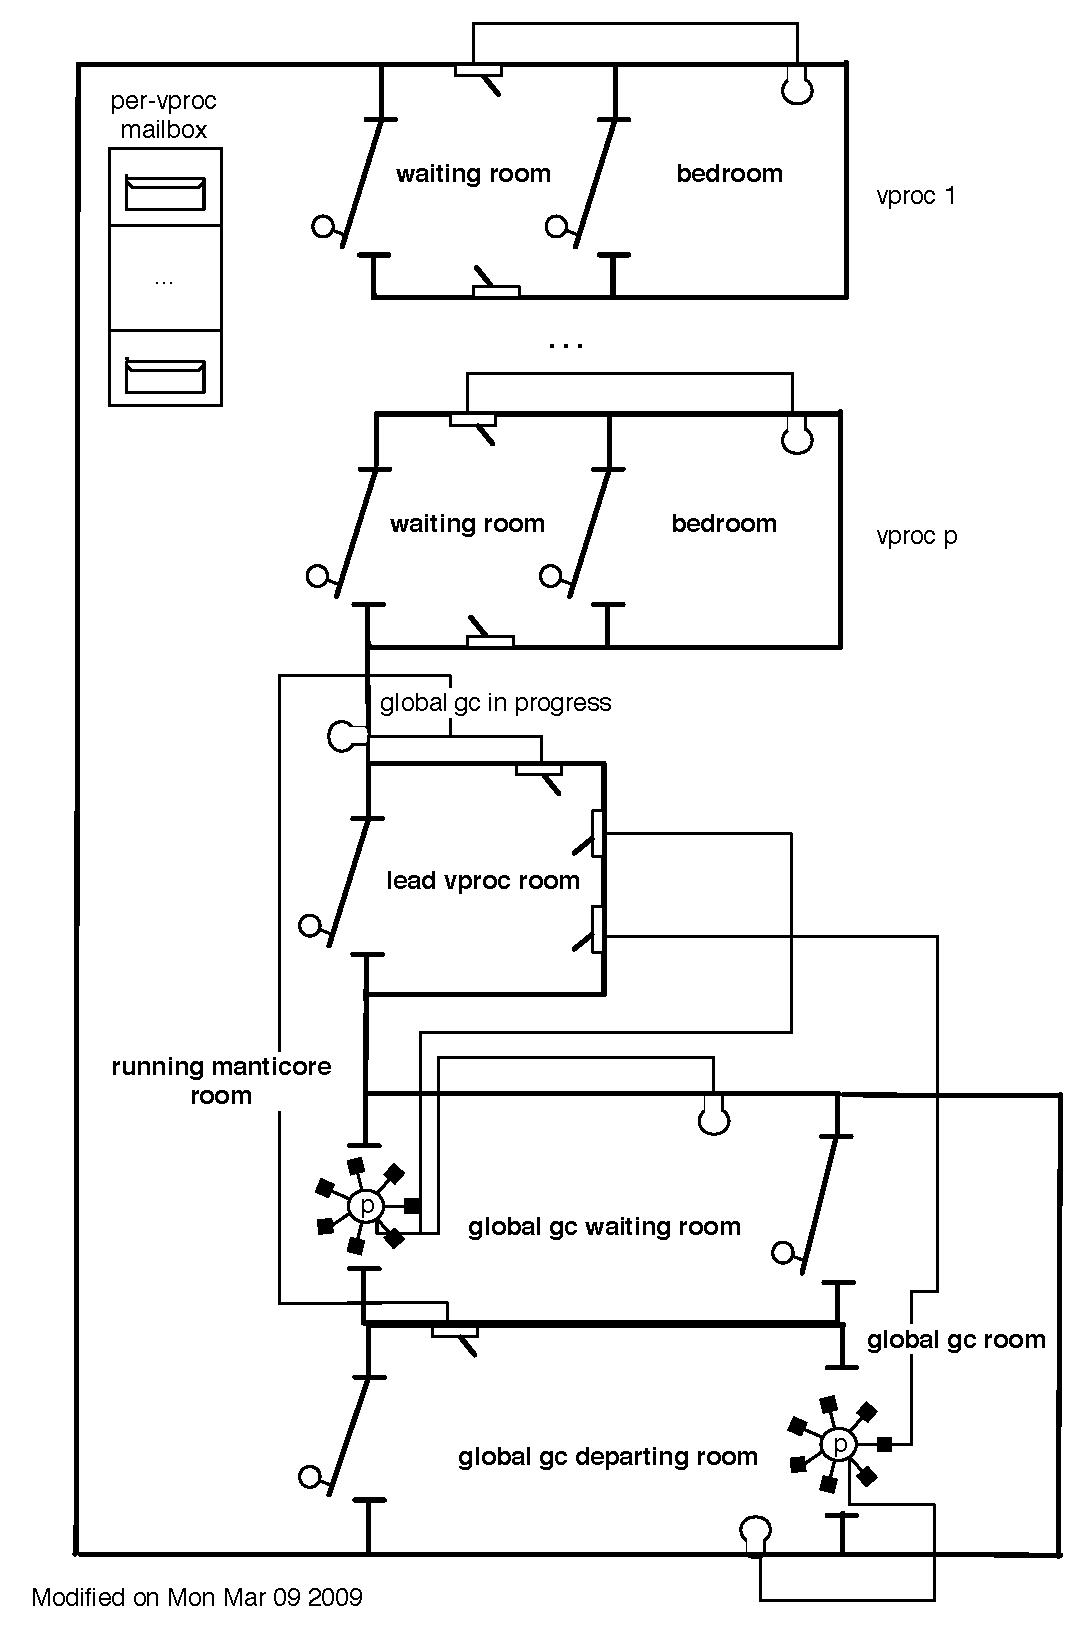
\includegraphics[scale=0.7]{pictures/vproc-protocol}
  \end{center}%
  \caption{Layout of the VProc protocol.}
  \label{fig:vproc-protocol}
\end{figure}%

\section{Messaging}

\paragraph{\texttt{Send(vp, msg)}}

\begin{description}
\item [\textit{Precondition:}] \textit{It is the case that} \texttt{vp} $\neq$ \texttt{host\_vproc} \textit{(a vproc cannot send a message to itself)}
\end{description}

\begin{enumerate}
  \item Walk to \texttt{vp}'s desk and open the mailbox.
    \begin{enumerate}
      \item If there is a \texttt{SLEEPING} message, place \texttt{msg} in the mailbox and go to step 2.
      \item Otherwise, place \texttt{msg} in the mailbox and exit the subroutine.
    \end{enumerate}
  \item Walk into \texttt{vp}'s \textbf{waiting room}.
    \begin{enumerate}
      \item If the waiting-room switch is off, then do the following. \textit{(\textbf{Invariant:}} \texttt{vp} \textit{is on its way to the waiting room.)}
        \begin{enumerate}
          \item Flip the waiting-room switch on.
          \item Return to the local desk.
          \item Exit the subroutine.
        \end{enumerate}
      \item If the waiting-room switch is on, then go to step 3. \textit{(\textbf{Invariant:}} \texttt{vp} \textit{is in its bedroom.)}
    \end{enumerate}
  \item Flip the bedroom switch on.
  \item Return to the local desk.
\end{enumerate}

\begin{description}
\item [\textit{Postcondition:}] \textit{At some point in the future,} \texttt{vp} \textit{will sit at its desk and open} \texttt{msg}.
\end{description}

\paragraph{\texttt{CheckMailbox()}}

\begin{enumerate}
  \item Open the local mailbox.
  \item Retrieve all messages, leaving the mailbox empty.
  \item Handle each message \texttt{msg}.
\end{enumerate}

\section{Sleeping}

\paragraph{\texttt{Sleep()}}

\begin{enumerate}
  \item Walk to the desk and open the mailbox.
    \begin{itemize}
      \item If empty, place a \texttt{SLEEPING} message in the mailbox.
      \item If nonempty, exit the subroutine.
    \end{itemize}
  \item Walk into the \textbf{waiting room}.
    \begin{itemize}
      \item If the waiting-room switch is on, then go to step 7. \textit{(\textbf{Invariant:}} \textit{Another vproc has delivered mail and has just walked out of the \textbf{waiting room}.)}
      \item If the waiting-room switch is off, then go to step 3. \textit{(\textbf{Invariant:}} \textit{It is the case that, in the time between the current step and step 1, no other vproc has entered the \textbf{waiting room}.)}
    \end{itemize}
  \item Flip the bedroom switch off.
  \item Walk into \textbf{bedroom}.
  \item Wait for the light to turn on.
  \item Walk into \textbf{waiting room}.
  \item Flip the waiting-room switch off.
  \item Return to the desk.
\end{enumerate}

\paragraph{\texttt{Wake(vp)}}

\begin{enumerate}
  \item Construct a blank message \texttt{msg}.
  \item Apply \texttt{Send(vp, msg)} and, once complete, exit the subroutine.
\end{enumerate}

\section{Global GC}

\paragraph{\texttt{GlobalLimit()}}

\begin{enumerate}
  \item Walk into \textbf{leader vproc room}.
    \begin{itemize}
      \item If switch is off, then we assign this vproc as the lead.
        \begin{enumerate}
          \item Flip the global-gc switch on.
          \item Reset turnstyles.
          \item Leave the \textbf{leader vproc room}.
          \item Go to \texttt{LeaderVProc()}.
        \end{enumerate}
      \item If switch is on, then go to step 2.
    \end{itemize}
  \item Walk into \textbf{global gc waiting room}.
  \item Wait for light to turn on.
  \item Enter \textbf{global gc room}.
  \item When finished with global collection, walk to \textbf{global gc departing room}.
  \item Wait for light to turn on.
  \item Return to the desk.
\end{enumerate}

\paragraph{\texttt{LeaderVProc()}}

\begin{enumerate}
  \item For each vproc \texttt{vp}, apply \texttt{Wake(vp)}.
  \item Walk into \textbf{global gc waiting room}.
  \item Wait for light to turn on.
  \item Walk into \textbf{global gc room}.
  \item When finished with global collection, walk to \textbf{global gc departing room}.
  \item Flip the switch off.
  \item Wait for light to turn on.
  \item Return to the desk.
\end{enumerate}
}

\end{document}  
